\documentclass[dvipdfmx]{jarticle}
\pagestyle{empty}
\usepackage{fancyvrb}
\usepackage{tikz}
\usetikzlibrary{shapes,calc,arrows.meta}
\begin{document}
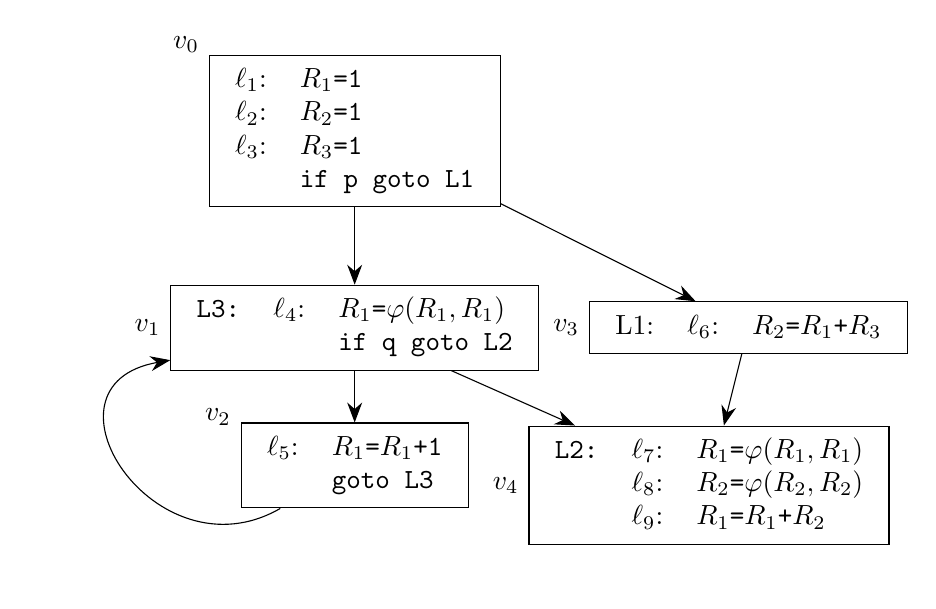
\begin{tikzpicture}
    \node[draw,rectangle,label={155:{$v_0$}}] (v0) at (0,0) {\begin{tabular}{ll}
            $\ell_1$: & $R_1$\verb|=1| \\
            $\ell_2$: & $R_2$\verb|=1| \\
            $\ell_3$: & $R_3$\verb|=1| \\
                    & \verb|if p goto L1|
        \end{tabular}};
    \node[draw,rectangle,label={180:{$v_1$}}] (v1) at (0,-2.5) {\begin{tabular}{lll}
            \verb|L3:| & $\ell_4$:  & $R_1$\verb|=|$\varphi(R_1,R_1)$\\
            & & \verb|if q goto L2|
        \end{tabular}};
    \node[draw,rectangle,label={165:{$v_2$}}] (v2) at (0,-4.25) {\begin{tabular}{ll}
            $\ell_5$: & $R_1$\verb|=|$R_1$\verb|+1| \\
            & \verb|goto L3|
        \end{tabular}};
    \node[draw,rectangle,label={180:{$v_3$}}] (v3) at (5,-2.5) {\begin{tabular}{lll}
            L1: & $\ell_6$: & $R_2$\verb|=|$R_1$\verb|+|$R_3$
        \end{tabular}};
    \node[draw,rectangle,label={180:{$v_4$}}] (v4) at (4.5,-4.5) {\begin{tabular}{lll}
            \verb|L2:| & $\ell_7$: & $R_1$\verb|=|$\varphi(R_1,R_1)$\\
                       & $\ell_8$: & $R_2$\verb|=|$\varphi(R_2,R_2)$\\
             & $\ell_9$: & $R_1$\verb|=|$R_1$\verb|+|$R_2$
        \end{tabular}};
    \path[-{Stealth[scale=1.5]}] (v0) edge (v1) (v0) edge (v3);
    \path[-{Stealth[scale=1.5]}] (v1) edge (v2) (v1) edge (v4);
    \path[-{Stealth[scale=1.5]}] (v3) edge (v4);
    \path[-{Stealth[scale=1.5]}] (v2) [out=210,in=190,looseness=2.0] edge (v1);
\end{tikzpicture}
\end{document}